\section{Sequence Model}
In this section, we discuss a another group of techniques which aims to process sequential or time series data, the case that data item may depend on the ones that precede or follow it. 
We begin by introducing the very basic sequence model, Recurrent Neural Network (RNN) and it's variants. After that, we present more complex and powerful techniques in language modeling. Finally, we introduce some popular toolkits that is widely applied in processing sequential data.
% \subsection{Sequence-to-sequence problem}
\subsection{Recurrent Neural Network}
Similar to the image modeling mentioned in previous section (\ref{model:cnn}), while the ConvNet focuses on learning embedding images, the goal of sequence model is to get a representation of a sequence. 
The Recurrent Neural Network (RNN) is improved upon the neural network which works on the principle of reserving the "memory" from prior input to influence current input and output. \\
RNN uses a hidden state as memory cell to capture the information processed so far. The model uses the same weight matrices throughout the sequence to process variable-length inputs.
Figure \ref{fig:rnn} shows how RNN processes a sequence. \\
Where $\mathbf{X} = [\mathbf{x_{1}}, \mathbf{x_{2}}, ..., \mathbf{x_{t}}, ..., \mathbf{x_{L}}]$ denotes a L-length input sequence. $\mathbf{h_{t}}$ is the hidden state at time $t$, which contains information from all of the past timesteps, contributes to the outcome $\mathbf{o_{t}}$ given current point $\mathbf{x_{t}}$. \\
Follow this approach, the final hidden state summarizes all the input information. Hence, the vector can be used as the representation for the whole input sequence. 
However, modeling this way contains an inevitable drawback. When the input is too long, the representation tends to "forget" and challenging to access the information from a long time ago.
\begin{figure}[t!]
    \centering
    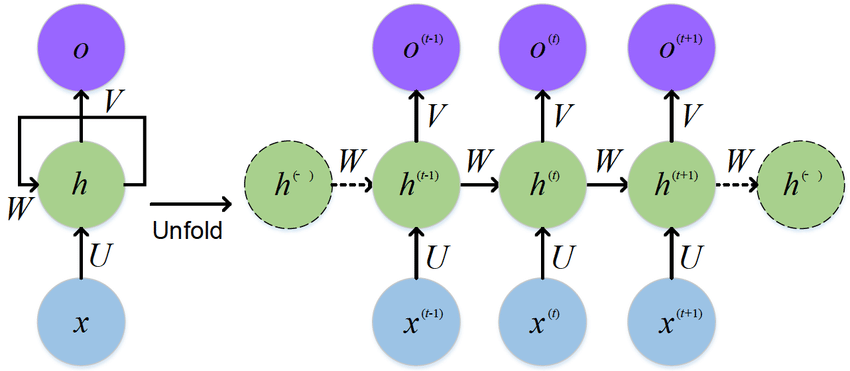
\includegraphics[width=0.8\textwidth]{images/RNN.png}
    \caption{Recurrent Neural Network architecture.}
    \label{fig:rnn}
\end{figure}
\subsection{Sequence-to-sequence model}
First introduced in \cite{sutskever2014sequence}, sequence-to-sequence (seq2seq) model targets to perform generating an output sequence from an input sequence, where both of them can have variable length. Some applications of seq2seq model include machine translation, question answering or text summarization, etc. \\
As proposed by its name, the architecture composes of two main branches:
\begin{enumerate}
    \item \textbf{Encoder} receives the input, processes and produces a context vector summarizing the whole input sequence
    \item \textbf{Decoder} achieves this embedded information to generate the appropriate output sequence word by word.
\end{enumerate}
Both Encoder and Decoder is built based on the RNN architecture. Figure ... shows an overview of this method. 
However, as mentioned above, the critical disadvantage of RNN representation is the capability of remembering long sentences, which could hugely damages the performance of seq2seq systems, such as translation machines. 
The model could easily forget those first words after encoding the entire input when working with a long document. 
This is when the attention mechanism \cite{bahdanau2014neural} comes into place.

\subsection{Attention Mechanism}
\label{sec:attention}
Intuitively, the attention mechanism core idea can be explained as follow. In machine translation problem, during the decoding process, the model should look back to source input each step to pick the most relative or important parts to make a good translation. 
For an example of how attention work, we solve a task of translate a source sentence $\mathbf{X}$ of length $n$ to a target sentence $\mathbf{Y}$ of length $m$. 
\begin{align*}
\mathbf{X} = [\mathbf{x_{1}}, \mathbf{x_{2}}, ..., \mathbf{x_{n}}] \quad \quad \quad
\mathbf{Y} = [\mathbf{y_{1}}, \mathbf{y_{2}}, ..., \mathbf{y_{m}}]
\end{align*}
where $\mathbf{x_{i}}$ denotes the embedding vector of the input $i^{th}$ word, $\mathbf{y_{i}}$ is the prediction vector of the output $i^{th}$ word. \\
Next, we adopt a basic RNN architecture for encoder $f_{E}$ and decoder $f_{D}$. At each time step $t$, encoder produce a single hidden vector $\mathbf{h_{t}}$.
The encoder first encoding the entire input source, result in list of n hidden states:
\begin{align*}
    \mathbf{h} = [\mathbf{h_1}, \mathbf{h_2}, ..., \mathbf{h_n}]
\end{align*}
The decoder iteratively compute hidden state $\mathbf{s_t} = f_D(\mathbf{s_{t-1}}, \mathbf{y_{t-1}}, \mathbf{c_t})$ used to predict output word $\mathbf{y_t}$ at timestep $t$ ($t = 1, 2, ..., m$). $\mathbf{c_t}$ is the context vector, given by the following formulas. 
% The context vector $\mathbf{c_t}$ stands for the looking back action used in prediction and can be computed through a sum of entire source hidden states $\mathbf{H}$, weighted by alignment score $\alpha_{t, i}$
\begin{align}
    \mathbf{c_t} &= \sum_{i=1}^{n} (\alpha_{t, i} \mathbf{h_i}) \label{eqn:attn_context} \\
    \alpha_{t, i} &= \frac{\mathrm{exp}(\mathrm{score}(\mathbf{s_{t-1}, \mathbf{h_i}}))}{\sum_{j=1}^{n}\mathrm{exp}(\mathrm{score}(\mathbf{s_{t-1}, \mathbf{h_j}})} \label{eqn:attn_score} 
\end{align}

In attention mechanism, to predict a new word, the model first need to decide which words of the input sentence to pay more attention on. This process is done through a function that score how well each encoded input matches the current output. These scores are then normalized and used as weights of importance for whole encoded units (function \ref{eqn:attn_score}). 
The final context representation at current time step is provided by a weighted sum of all encoder hidden states, formulated in \ref{eqn:attn_context}.
 
\begin{table}[h]
\centering
\caption{Summary of several score functions used in attention mechanism. }
\footnotesize
\begin{tabular}{ c | c | c  }
\hline
\textbf{Name} & \textbf{Score function} & \textbf{Citation} \\
\hline
Additive & $ \mathrm{score}(\mathbf{s_t}, \mathbf{h_i}) = \mathbf{v}^T \mathrm{tanh}(\mathbf{W}[\mathbf{s_t}, \mathbf{h_i}])$  & 	Bahdanau et al. \cite{bahdanau2014neural}  \\
Dot-Product &  $\mathrm{score}(\mathbf{s_t}, \mathbf{h_i}) = \mathbf{s_t}^T \mathbf{h_i}$ & Luong et al. \cite{luong2015effective} \\ 
Scaled Dot-Product & $\mathrm{score}(\mathbf{s_t}, \mathbf{h_i}) = \frac{\mathbf{s_t}^T \mathbf{h_i}}{\sqrt{n}} $ & Vaswani et al.\cite{vaswani2017attention} \\
\hline
\end{tabular}
\label{table:attn_score}
\end{table}
The $\mathrm{score}$ function in \ref{eqn:attn_score} computes the similarity between two same-length vectors. Hence, there are several scoring functions were proposed to improve this technique (shown in table \ref{table:attn_score}). Bahdanau et al.\cite{bahdanau2014neural} first introduced a trainable score function, which is parameterized by a feed-forward neural network. Luong et al.\cite{luong2015effective} proposed a simpler one, the dot-product scoring function, and showed to get better performance. Vaswani et al scaled down the dot-product by the vector size to handle the issue that softmax function provides extremely small gradient when the input is large.
%where $\mathbf{W}, \mathbf{v} $ are trainable weights
%where $n$ is size of the source hidden state & Vaswani et al

The attention mechanism has given a big improvement in sequence modeling. Not only in machine translation, the technique has also proved to perform well on variety tasks. 
Therefore, many researches surveyed other forms of attention applying to seq2seq problems and arrived at potential results.
In 2017, Vaswani et al.\cite{vaswani2017attention} proposed a novel model based solely on attention machanisms, without using any recurrent architectures, and outperforms almost RNN-based methods at that time. In the next section, we briefly introduce the transformer architecture, which is currently applied in almost sequence modeling problems and achieve potential results.

\subsection{Transformer}
\label{sec:transformer}
The core idea behind transformer architecture is the self-attention mechanism to produce a better representation of the sequence itself. 
We first mathematically show how the self-attention work, then introduce some major concepts used to construct the complete model. 
Finally, we explain how transformer work as an encoder-decoder architecture for seq2seq problems. 
\subsubsection{Self-attention}
\label{sec:self_attn}
Self-attention is an variant of the original attention technique discussed in section \ref{sec:attention}, which provide the ability to attend to different parts of the input sequence. Given a set of $t$ elements, the module returns $t$ representations for each unit respectively.
Essentially, for a $t$-length input sequence
\begin{align*}
    \mathbf{X} = \{{\mathbf{x_i}}\}_{i=1}^t = \{\mathbf{x_1}, \mathbf{x_2}, ..., \mathbf{x_t}\}
\end{align*}
where each $\mathbf{x_i}$ is the embedded input element with $n$ dimension, hence we have $\mathbf{X} \in \mathbb{R}^{n \times t}$.
Each element will then have a corresponding attention weight $\mathbf{a_i}$ with regards to the whole input sequence ($\mathbf{a_i} \in \mathbb{R}^t$). This weight is formulated as:
\begin{align}
    \label{eqn:self_attn_alpha}
    \mathbf{a_i} = \mathrm{softmax}(\mathbf{X}^T\mathbf{x_i})
\end{align}
The representation of the $i$-th input unit is the linear combination of whole input embeddings:
\begin{align}
    \mathbf{h_i} =  \mathbf{X}\mathbf{a_i}
\end{align}
Apply the process for all input elements, we obtain a set of representations $\mathbf{H} \in \mathbb{R}^{n \times t}$. In the next session, we introduce how transformer utilizes self-attention to encode input and produce output as an encoder-decoder structure.
\begin{figure}[t!]
    \centering
    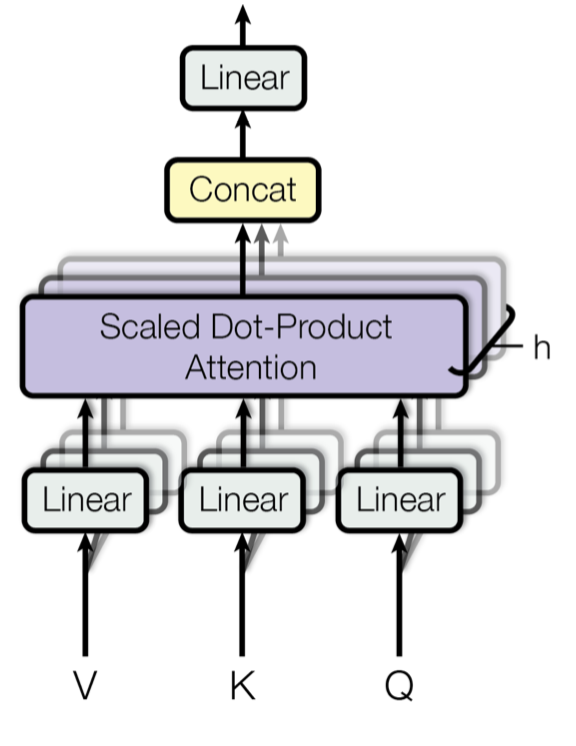
\includegraphics[width=0.4\textwidth]{images/Transformer_multi-head.png}
    \caption{Multi-head scaled dot-product attention mechanism.\cite{vaswani2017attention}}
    \label{fig:trans_multi-head}
\end{figure}
\subsubsection{Queries, keys and values}
Intuitively, when we are looking for new terminologies in a book, one of the most convenient way is to compare our words with each line of the content page, then pick those most related contents based on how their titles match with our needs. The new terminology here is our \textit{query}, which is then compared against all \textit{keys} (titles) in the dataset to retrieve most similar \textit{values} (contents).
This idea demonstrates how the transformer encoder, decoder works.\\
Transformer views the input sequence as a dictionary, where each embedded element is a \textit{key-value} pair, and both these keys and values are the encoder hidden states.
In decoder, previous output is utilized as \textit{query} to check on the input's key-value information to predict the next output. In encoder, to obtain representation for the input itself, \textit{query} is generated from the input embedding, and the process works as follow. \\
The first step is to create three vectors for each embedded input vector $\mathbf{x_i}$, a \textit{query} vector, a \textit{key} vector and a \textit{value} vector as follow.
\begin{align*}
    \mathbf{q_i} &= \mathbf{W_q}\mathbf{x_i} \\
    \mathbf{k_i} &= \mathbf{W_k}\mathbf{x_i} \\
    \mathbf{v_i} &= \mathbf{W_v}\mathbf{x_i}
\end{align*}
where $\mathbf{W_q}, \mathbf{W_k}, \mathbf{W_v}$ are both learnable parameters. And $\mathbf{q}$ and $\mathbf{k}$ must have the same dimensionality. But value vector $\mathbf{v}$ can have arbitrary length. For simplicity, we set dimension of both query, key and value to $d$. Stacking these vectors of the entire input, we obtain $\mathbf{Q}, \mathbf{K}, \mathbf{V} \in \mathbb{R}^{d \times t}$. \\
Now, to find the necessary content, we compare our queries $\mathbf{q_i}$ to all possible keys $\mathbf{K}$ to gain a vector of matching scores.
\begin{align}
    \mathbf{a_i} = \mathrm{softmax}(\frac{\mathbf{q_i}\mathbf{K}^T}{\sqrt{d}})
\end{align}
The term $\frac{1}{\sqrt{d}}$ here indicates that scale dot-product scoring function is adapted in transformer. 
Now, we obtain $t$ corresponding weights $\mathbf{a_i}$ for each query, which forms a matrix $\mathbf{A} \in \mathbb{R}^{t \times t}$
Similar to \ref{sec:self_attn}, the final representation of these input elements are obtained through a linear combination of all values $\mathbf{V}$ weighted by it's score $\mathbf{a_i}$.
\begin{align}
    \mathbf{H} = \mathbf{A} \mathbf{V} = \mathrm{softmax}(\frac{\mathbf{Q}\mathbf{K}^T}{\sqrt{d}}) \mathbf{V}
\end{align}
In transformer, each triplet of transformations $[\mathbf{W_q}, \mathbf{W_k}, \mathbf{W_v}]$ is called a \textit{head}. 
And we could use multiple heads to construct a deeper modeling. The independent outputs from each head are concatenated and linearly transformed to the final representation with appropriate dimension. This is called the \textit{multi-head self-attention} technique in the transformer setting. 
Figure \ref{fig:trans_multi-head} illustrates the workflow of this module.

\subsubsection{Encoder-Decoder architecture}
\begin{figure}[t!]
     \centering
     \subfloat[Encoder block.]{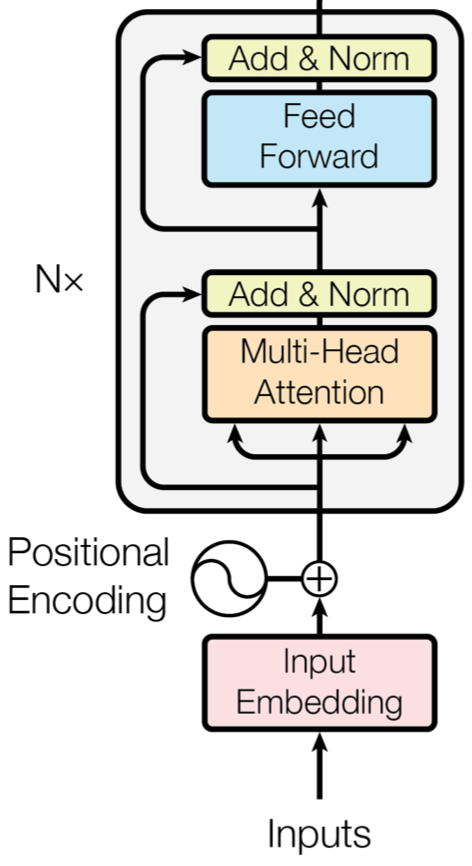
\includegraphics[width=0.3\textwidth]{images/transformer_encoder.png}\label{fig:trans_enc}}
     \hspace{2cm}
     \subfloat[Decoder block]{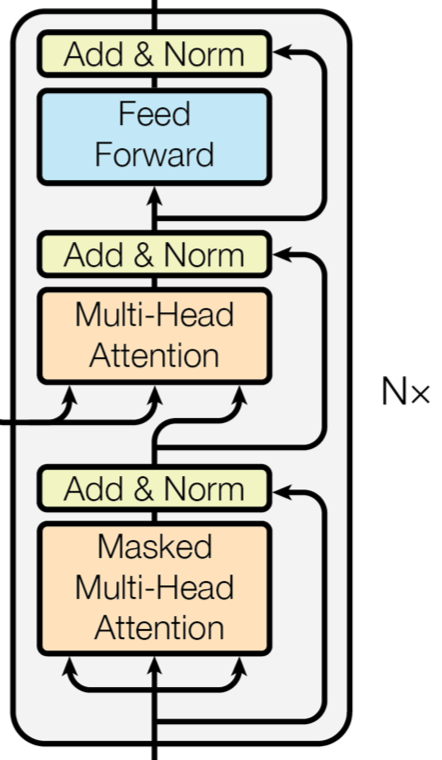
\includegraphics[width=0.3\textwidth]{images/transformer_decoder.png}\label{fig:trans_dec}}
     \caption{The Transformer Encoder, Decoder architecture.\cite{vaswani2017attention}}
     \label{fig:trans_enc_dec}
\end{figure}
In this session, we go through how encoder, decoder blocks of transformer are constructed (illustrated in figure \ref{fig:trans_enc_dec}).\\
The \textbf{encoder} receives a set of inputs $\{{\mathbf{x_i}}\}_{i=1}^t$ and outputs a set of hidden states $\{{\mathbf{h_i^{e}}}\}_{i=1}^t$. The module is built from $N$ encoder blocks, each block includes a multi-head self-attention layer following by a fully-connected network. These layers both adopt residual connection and a normalization for better training. \\
The \textbf{decoder} follows a similar procedure as the encoder, but adds one multi-head self-attention layer to compress the previous outputs as \textit{queries} for next output prediction. The key-value pairs are still the encoder hidden states. Therefore, this procedure is also called \textit{cross-attention}.  

\subsection{BERT}
\label{sec:BERT}
In the area of natural language processing, pre-trained models have been shown to be convenient and efficient to apply in many different tasks, such as sentence-level tasks (text summarization \cite{jadhav2018extractive, liu2018generative}, paraphrase generation \cite{wieting2017paranmt}, etc.) or token-level tasks (semantic role labeling \cite{he2018jointly,shi2019simple}, named entity recognition \cite{baevski2019cloze,strakova2019neural}, etc.). In this section, we introduce a language representation model that was widely used as a pretrained backbone or fine-tuned for various tasks to achieve potential results, namely BERT (Bidirectional Encoder Representations from Transformer) \cite{devlin2018bert}. Figure \ref{fig:BERT_finetune} shows some tasks finetuned from BERT backbone.
\begin{figure}[t!]
    \centering
    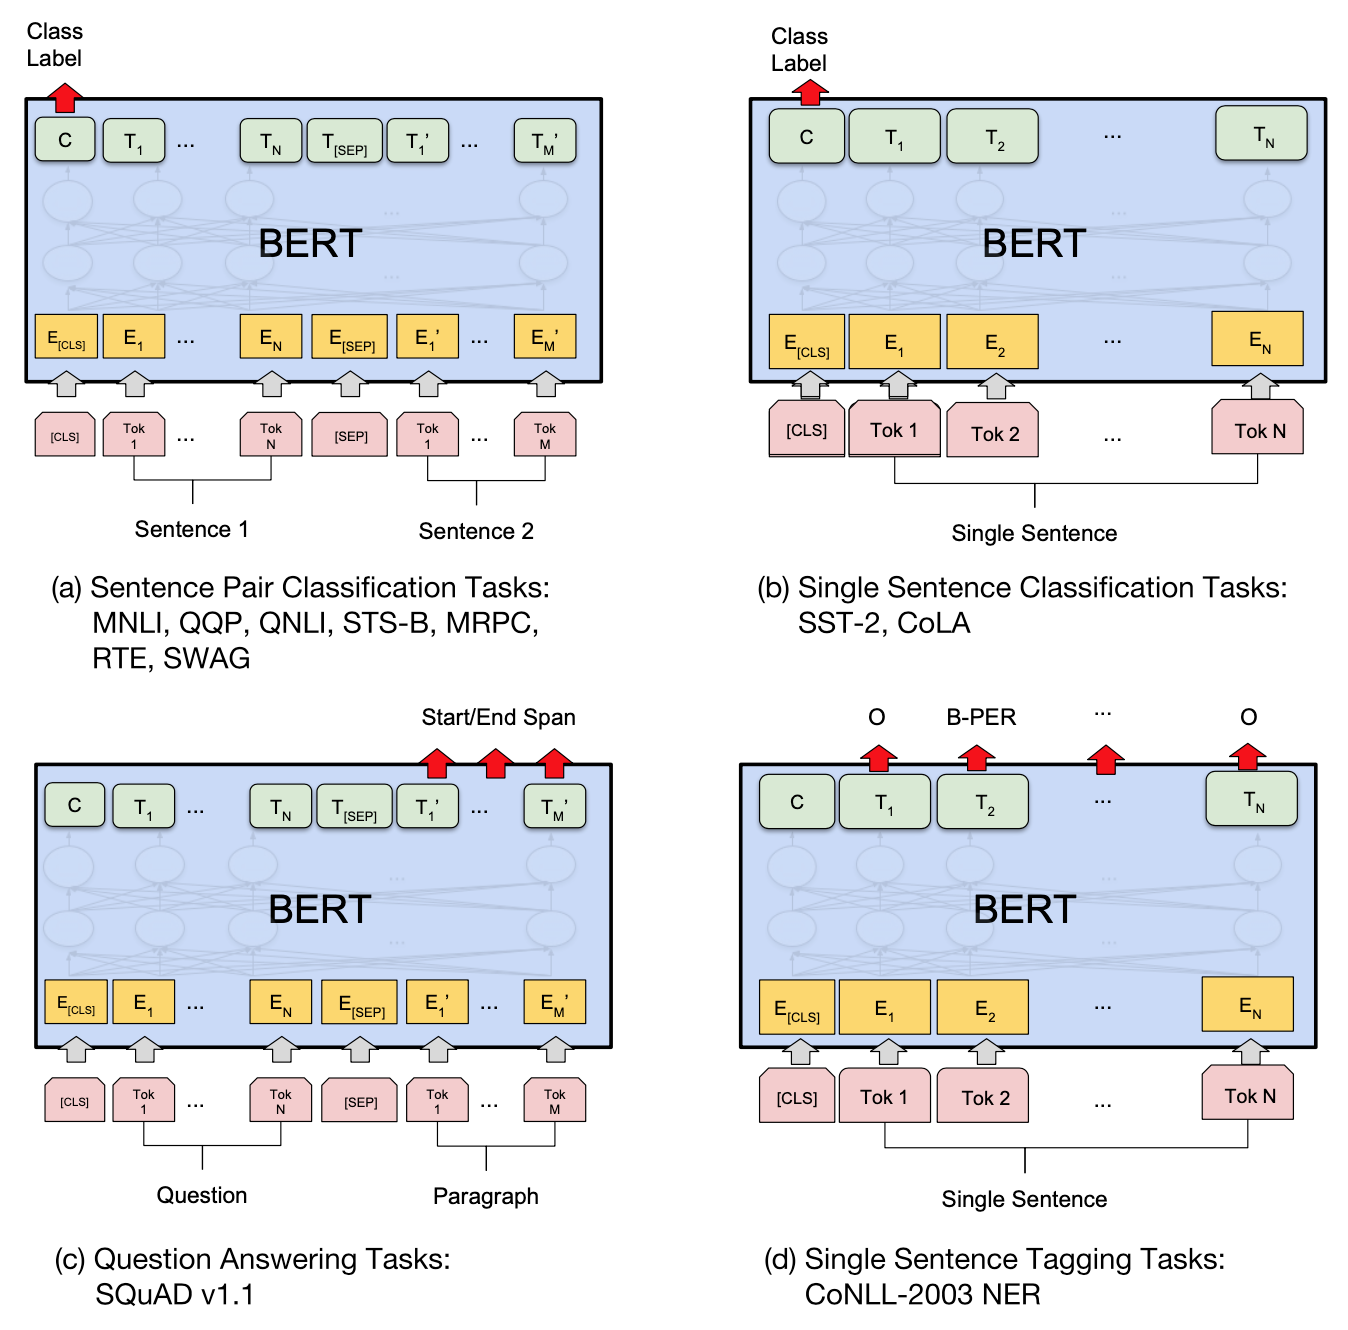
\includegraphics[width=0.9\textwidth]{images/BERT_finetune.png}
    \caption{Examples of finetuning BERT on common tasks with different types of input. \cite{devlin2018bert}}
    \label{fig:BERT_finetune}
\end{figure}
\textbf{Architecture details}. \\
As the name suggests, the BERT model learns the bidirectional text representation by a stack of $L$ transformer encoder blocks (section \ref{sec:transformer}), $A$ self-attention heads for the $H$-length hidden representation. These parameters indicate two different versions of BERT: 
\begin{itemize}
    \item $\mathbf{BERT_{BASE}}$: $L = 12, H = 768, A = 12$, total parameters $= 110M$
    \item $\mathbf{BERT_{LARGE}}$: $L = 24, H = 1024, A = 16$, total parameters $= 340M$
\end{itemize}

\subsubsection{Input representation}
In the preprocessing stage, BERT tokenizes input words with WordPiecing embedding \cite{wu2016google} to handle the unknown words problem. Out-of-vocabulary (OOV) words are broken into subwords greedily. For example, the word ‘judgemental’ is OOV, tokenizer splits it into ‘judgment’ and ‘\#\#al’, here ‘\#\#’ indicates subwords. Therefore, this technique ensures that every input word is constructed from some forms of wordpieces, instead of converting all OOV words to an unknown token.
Additionally, BERT tokenizer introduces several tokens used for better modeling.
\begin{itemize}
    \item {[CLS]}: The special classification token, stands first in every input sequence, used in classification task as an aggregate of the entire sequence representation. The token is ignored in non-classification task.
    \item {[SEP]}: The separator token used to separate two distinct sentences or mark for the end of a sentence.
    \item {[MASK]}: This token is used in pre-training stage with masked language modeling.
    \item {[PAD]}: This token is used to pad the input sequence with a shorter length than pre-defined BERT input size.
\end{itemize}
Figure \ref{fig:BERT_input} shows an example of this process.
\begin{figure}
    \centering
    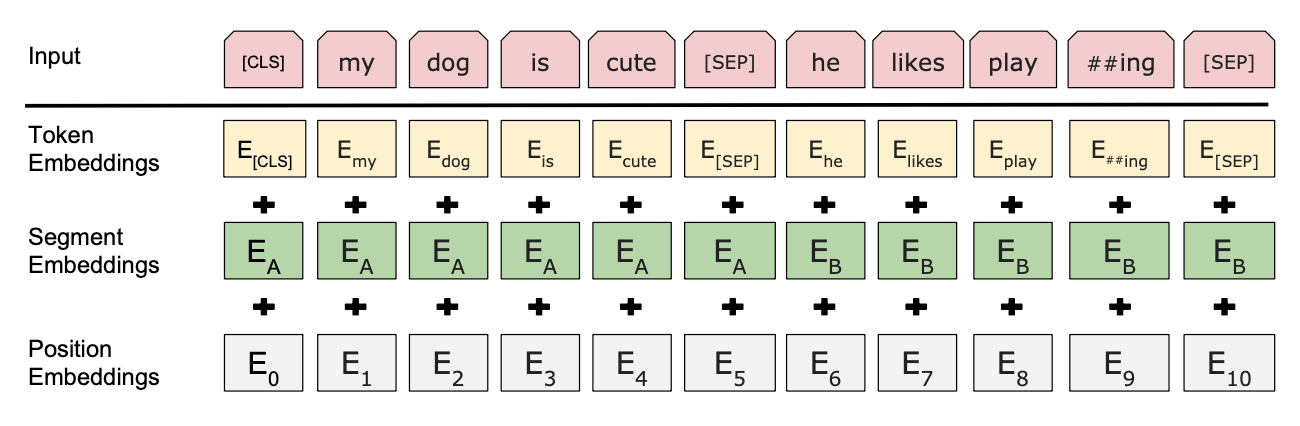
\includegraphics[width=0.9\textwidth]{images/BERT_input.png}
    \caption{An example of BERT input representation process \cite{devlin2018bert}.}
    \label{fig:BERT_input}
\end{figure}
\subsubsection{Pretraining BERT}
BERT is introduced to provide a powerful pretraining backbone to handle various downstream tasks. To reach this goal, the model is pre-trained through two unsupervised tasks called Next Sentence Prediction (NSP) and Masked Language Modeling (MLM), which learns different features of the input sequence.

\textbf{Masked Language Modeling} \\ 
The Language Model process \cite{dai2015semi} task aims at predicting the next word using previous sequence words to help language models learn better representations (ELMo \cite{peters2018deep}, OpenAI GPT \cite{radford2018improving}).
Different from those directional predictions, where the task is trained in left-to-right or right-to-left through the sequence, each unit in BERT is connected to the whole context in all layers with the self-attention mechanism. Therefore, to solve the MLM task, the author uses a Masked Language Model to randomly mask some percentage (15\%) of the inputs as follows: \\
80\% of the time replace the word with the [MASK] token. \\
10\% of the time replace the word with with another random token. \\
10\% of the time do nothing, ignore the replacement.

\textbf{Next Sentence Prediction} \\
This task performs the binary classification to answer the question of if the two sentences are following each other or not. Intuitively, while the MLM helps the model to learn relationships between words in a sentence, NSP provides a sentence-level relationships understanding. The training dataset contains a bunch of pairs (sentence A, sentence B). In 50\% of the samples, sentence B is truly following sentence A while in the other 50\%, sentence B is randomly selected from the corpus.



